\section{Theorie}\label{sec:theorie}

\subsection{Kristallgitter}\label{subsec:kristallgitter}
Um das Material \heo, sowie die Röntgendiffraktometrie verstehen zu können, ist ein grundlegendes Verständnis
über die Struktur kristalliner Festkörpern unerlässlich.
Die nachfolgenden Seiten dienen deshalb als Zusammenfassung der für die Arbeit relevanten Konzepte der Festkörperphysik.

\subsubsection{Bravaisgitter, Elementarzelle und Basis}
Als Idealisierung vieler Festkörper wird das Modell des idealen Kristalls herangezogen.
Laut \citeauthoryear{Hunklinger} ist ein idealer Kristall eine dreidimensionale, unendlich ausgedehnte Anordnung,
die sich aus identischen, periodisch wiederkehrenden Baueinheiten zusammensetzt.
Diese Baueinheiten werden als Basis bezeichnet.
Sie können einzelne Atome, aber auch komplexe Atomstrukturen repräsentieren.
Reduziert man jede Baueinheit auf einen einzigen Punkt, so entsteht ein einfach zu beschreibendes Punktgitter.
Dieses unterliegt verschiedenen Symmetrien, sodass das Gitter in unterschiedliche Kristallsysteme eingeteilt werden
kann.
Eine einfache Einteilung kann mithilfe von Drehachsen erfolgen.
Hierbei betrachtet man diejenigen Rotationsoperatoren $R_{\hat{e}}(2\pi / n)$ für eine beliebige Achse $\hat{e}$ um
einen Winkel $2 \pi /n$, die das Punktgitter auf sich selbst abbilden.
Der Parameter $n \in \mathbb{N}$ wird als Zähligkeit bezeichnet und teilt die Punktgitter in sieben verschiedene
Kristallklassen ein, die in \cref{tab:krystallsysteme} aufgeführt sind \autocite{Hunklinger}.

\begin{table}[h]
    \centering
    \begin{tabular}{c c c c}
        \toprule
        Kristallsystem           & Gitterkonstanten  & Winkel                                       & Zähligkeit \\ \midrule
        triklin                  & $a \neq b \neq c$ & $\alpha \neq\beta \neq\gamma$                & 1          \\
        monoklin                 & $a \neq b \neq c$ & $\alpha=\gamma=\ang{90},\beta \neq \ang{90}$ & 2          \\
        orthorhombisch           & $a \neq b \neq c$ & $\alpha=\beta=\gamma=\ang{90}$               & 2 (zwei)   \\
        tetragonal               & $a = b \neq c$    & $\alpha=\beta=\gamma=\ang{90}$               & 4          \\
        hexagonal                & $a = b \neq c$    & $\alpha=\beta=\ang{90}, \gamma=\ang{120}$    & 6          \\
        trigonal (rhomboedrisch) & $a=b=c$           & $\alpha=\beta=\gamma \neq \ang{90}$          & 3          \\
        kubisch                  & $a=b=c$           & $\alpha=\beta=\gamma=\ang{90}$               & 3 (vier)   \\ \bottomrule
    \end{tabular}
    \caption{Klassifikation der verschiedenen Kristallsysteme. \imcite{Hunklinger} }
    \label{tab:krystallsysteme}
\end{table}

Eine weitere wichtige Symmetrie ist die Translationssymmetrie.
Betrachtet man diejenigen Translationsoperatoren $T(\mathbf{O})$, die das Gitter auf sich selbst abbilden, dann erkennt
man aufgrund der Periodizität des Gitters den Zusammenhang
$\mathbf{O} = n_{1}\mathbf{a}_{1}+n_{2}\mathbf{a}_{2}+n_{3}\mathbf{a}_{3}$, wobei
$\mathbf{a}_{i}\in\mathbb{R}^{3}, n_{i}\in\mathbb{Z}, i\in \{1,2,3\}$ \autocite{Hunklinger}.
Die Vektoren $\mathbf{a}_{i}$
definieren ein schiefwinkliges Koordinatensystem und werden als primitive Gittervektoren bezeichnet.
Sie spannen ein dreidimensionales Bravaisgitter auf.
Die Abstände zwischen zwei benachbarten Gitterpunkten, also die Größen
$\lvert \mathbf{a}_{i} \rvert$, werden Gitterkonstanten genannt \autocite{Ashcroft}.
Je nachdem, wie sich das Kristallsystem unter Symmetrieoperationen verhält, ergeben sich unterschiedliche Bedingungen für
Gitterkonstanten und die Winkel zwischen den Gittervektoren.
Mithilfe der Definition einer Basis und eines Bravaisgitters lässt sich jeder ideale Kristall beschreiben.
Eine Kristallstruktur wird durch identische Kopien der Basis an jedem Punkt des Bravaisgitters aufgebaut
\autocite{Ashcroft}.


Laut \citeauthoryear{Ashcroft} kann durch geschickte Wahl von Teilmengen des Ortsraumes der gesamte Ortsraum durch
überlappungsfreie Aneinanderreihung der Teilmengen lückenlos gefüllt werden.
Solche Mengen nennt man Elementarzellen.
Wählt man die Elementarzelle so, dass sie nur einen Gitterpunkt enthält, spricht man von einer primitiven
Elementarzelle.
Mit einer primitiven Elementarzelle lässt sich der Raum lückenlos und überlappungsfrei überdecken, indem man die Zelle
entlang jedes Bravaisgittervektors verschiebt.
Eine einfache Konstruktion liefert ein Parallelepiped, welches von den drei Basisvektoren aufgespannt wird.
Das Volumen $V_\mathrm{EZ}= \lvert \mathbf{a}_1 \cdot (\mathbf{a}_2 \times  \mathbf{a}_3) \rvert$ dieses
Parallelepipeds gibt das effektive Volumen pro Bravais-Gitterpunkt an \autocite{Ashcroft}.


Eine weitere Unterteilung der Kristallsysteme kann mithilfe der dreidimensionalen Bravaisgitter erfolgen.
Diese lassen sich durch Operationen der Punktgruppe erzeugen und kategorisieren periodische Strukturen
in 14 verschiedene Bravaisgitter \autocite{Grundmann}.
Die für die Arbeit relevanten Gitter werden im Folgenden vorgestellt.

\subsubsection{Ausgewählte Kristallgitter}\label{subsubsec:kristallgitter}
\begin{figure}
    \centering
    \begin{subfigure}[t]{0.3\textwidth}
        \centering
        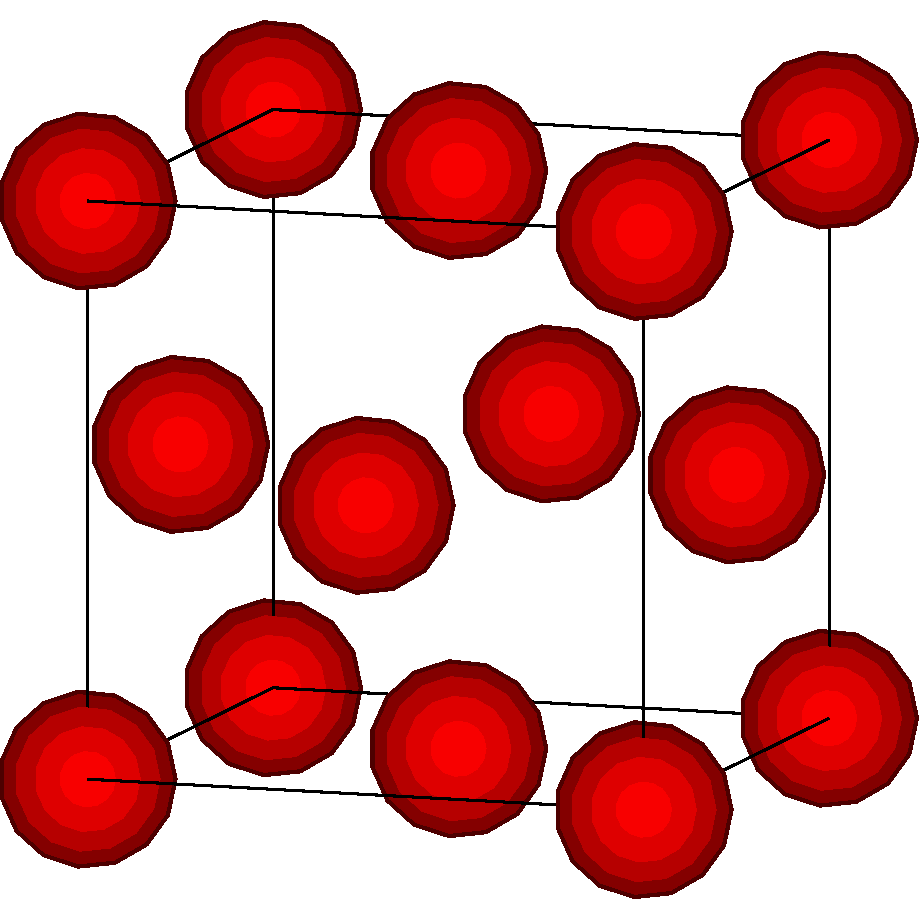
\includegraphics[width=\textwidth]{../assets/theorie/fcc}
        \caption{fcc-Gitter.} \label{fcc}
    \end{subfigure}
    \begin{subfigure}[t]{0.3\textwidth}
        \centering
        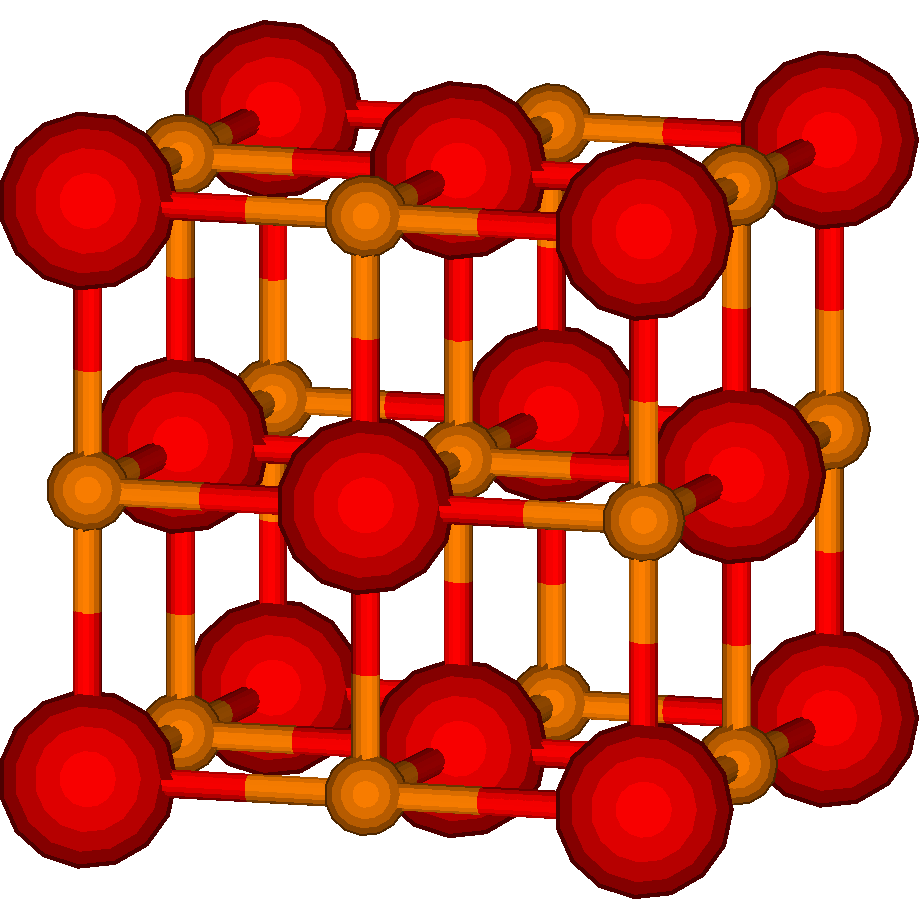
\includegraphics[width=\textwidth]{../assets/theorie/rocksalt}
        \caption{NaCl-Gitter} \label{nacl}
    \end{subfigure}
    \begin{subfigure}[t]{0.3\textwidth}
        \centering
        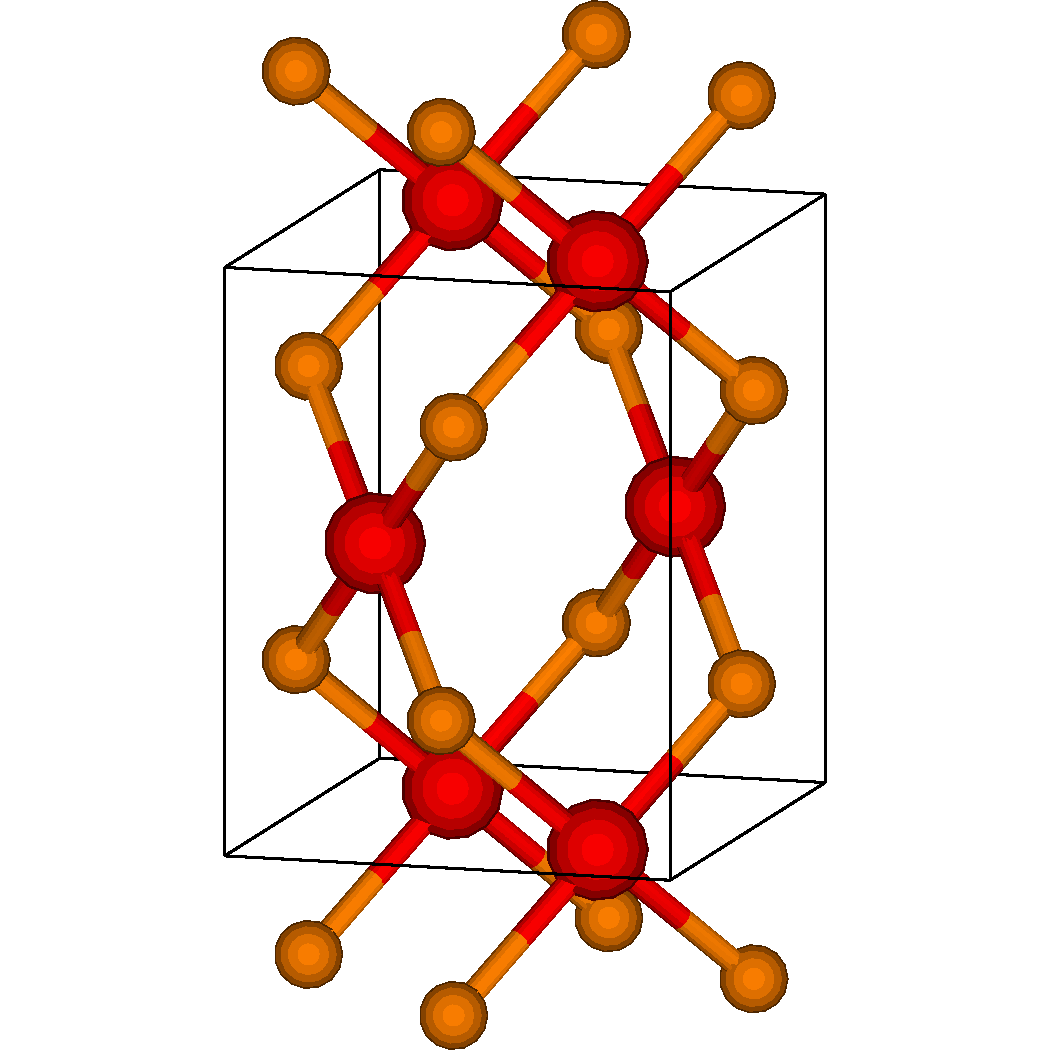
\includegraphics[width=\textwidth]{../assets/theorie/CuO}
        \caption{\ce{CuO}-Gitter} \label{cuo}
    \end{subfigure}
    \begin{subfigure}[t]{0.3\textwidth}
        \centering
        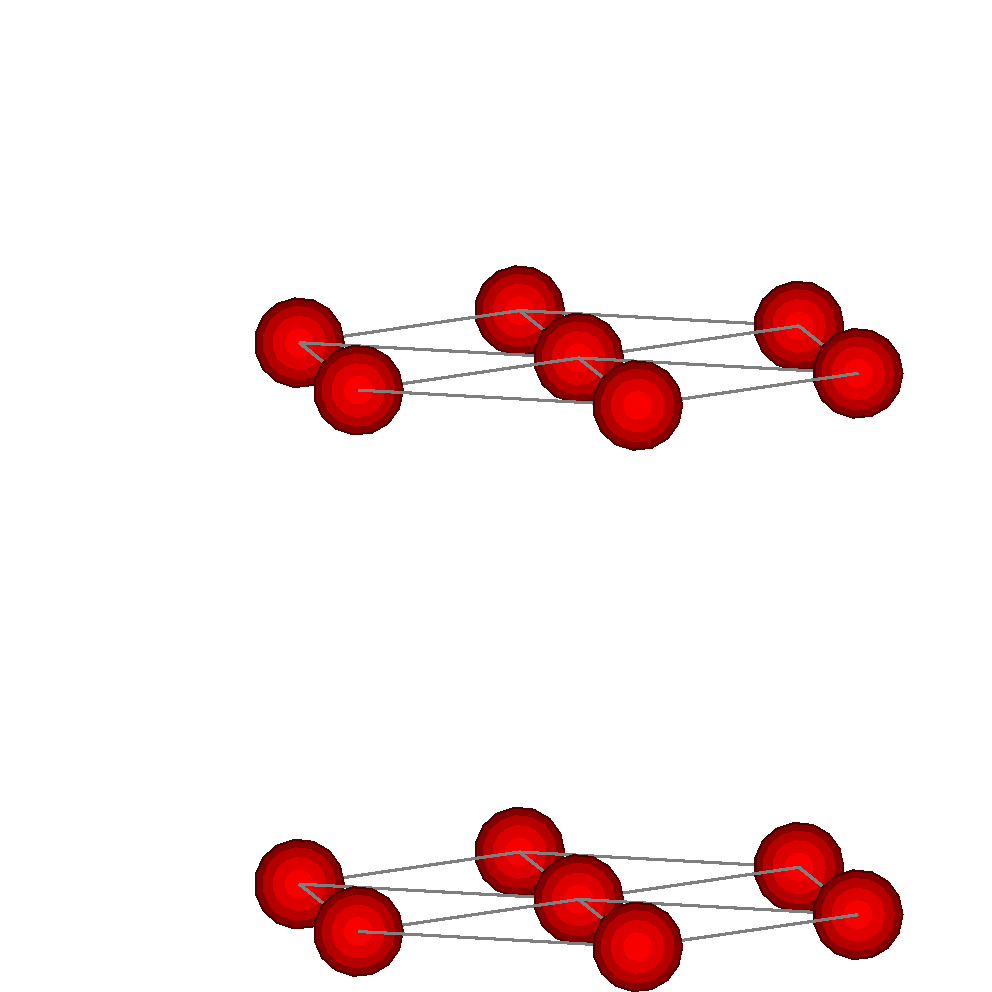
\includegraphics[width=\textwidth]{../assets/theorie/hex}
        \caption{hexagonales Gitter} \label{hex}
    \end{subfigure}
    \begin{subfigure}[t]{0.3\textwidth}
        \centering
        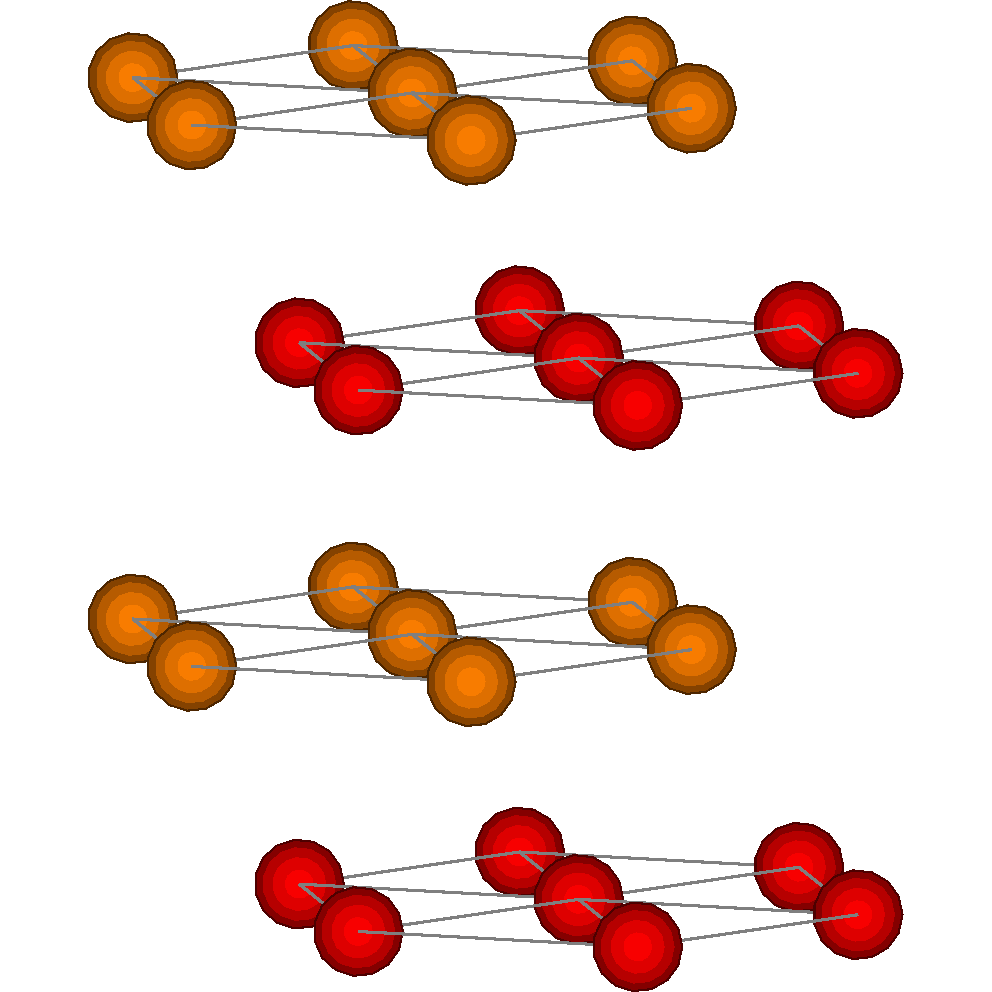
\includegraphics[width=\textwidth]{../assets/theorie/hcp}
        \caption{hcp-Gitter} \label{hcp}
    \end{subfigure}
    \begin{subfigure}[t]{0.3\textwidth}
        \centering
        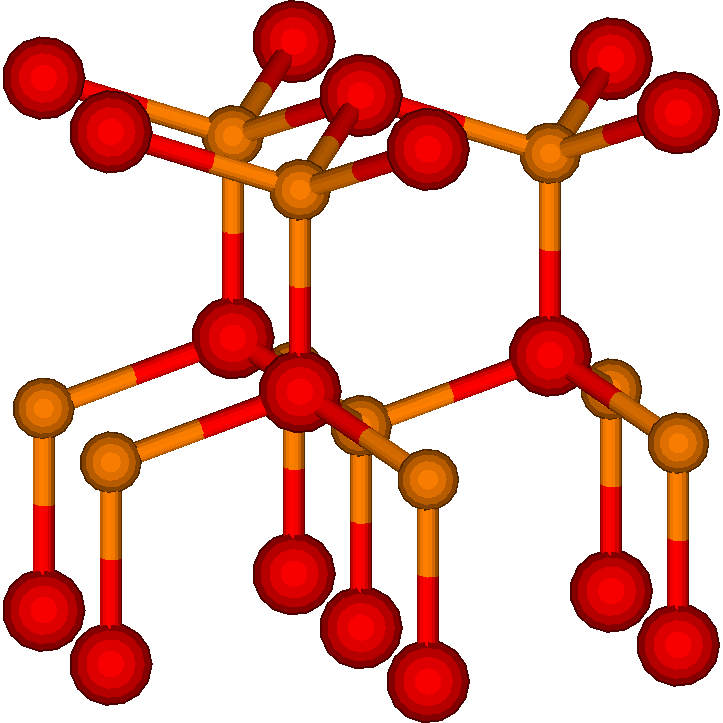
\includegraphics[width=\textwidth]{../assets/theorie/wurzite}
        \caption{Wurtzit-Gitter} \label{wurtzit}
    \end{subfigure}
    \caption{Ausgewählte Kristallgitter für die Untersuchung von \heo.} \label{fig:gitterstrukturen}
\end{figure}

\paragraph{Natriumchloridstruktur}
Die erste und wichtigste Kristallstruktur ist die Natriumchloridstruktur.
Um diese zu verstehen, betrachtet man zuerst ein kubisch-flächen\-zen\-trier\-tes Gitter (fcc, engl.
\textit{face-centered cubic}) welches durch die primitiven Vektoren
\begin{equation}
    \mathbf{a}_1 = a / 2 (\hat{x} + \hat{y}), \quad
    \mathbf{a}_2 = a / 2 (\hat{y} + \hat{z}), \quad
    \mathbf{a}_3 = a / 2 (\hat{x} + \hat{z})
    \label{eq:fcc}
\end{equation}
definiert ist \autocite{Grundmann}.
Die Gitterpunkte liegen an Würfelecken und den dazugehörigen Flächenmittelpunkten, wie in \cref{fcc} dargestellt.
Die Natriumchloridstruktur entsteht aus einem fcc-Gitter mit zweiatomiger Basis \autocite{Grundmann}.
Dabei ist das erste Basisatom an der Gitterposition $(0,0,0)$ und das zweite an der Position $(a/2,a/2,a/2)$, wie in
\cref{nacl} dargestellt.
Sowohl Magnesiumoxid (\ce{MgO}), Kobaltoxid (\ce{CoO}) und Nickeloxid (\ce{NiO}) kristallisieren in dieser Struktur.
Auch \heo\ kristallisiert in der Natriumchloridstruktur, wenn
Sauerstoff als erstes Basisatom und ein zufällig ausgewähltes Metall als zweites Basisatom betrachtet werden
\autocite{Rost2015}.

\paragraph{Tenoritstruktur}
Kupferoxid (\ce{CuO}) kristallisiert in einer monoklinen Kristall\-struk\-tur mit achtatomiger Basis.
Dabei sind vier dieser Basisatome Kupferatome und vier Sauerstoffatome.
Die Struktur ist in \cref{cuo} dargestellt \autocite{kupferoxid}.

\paragraph{Wurtzitstruktur}
Um die Wurtzitstruktur zu verstehen, betrachtet man zuerst die einfach-hexagonale Struktur, die durch die primitiven
Vektoren
\begin{equation}
    \mathbf{a}_1 = a\hat{x}, \quad
    \mathbf{a}_2 = a/2 (\hat{x} + \sqrt{3} \hat{y}), \quad
    \mathbf{a}_3 = c \hat{z}
    \label{eq:hex}
\end{equation}
definiert ist \autocite{Ashcroft}.
Es entsteht ein Gitter, welches an den Ecken eines Sechsecks und den dazugehörigen Flächenmittelpunkten Gitterpunkte
besitzt, wie in \cref{hex} dargestellt.
Aus der einfach-hexagonalen Struktur ergibt sich die hexagonal dichtest gepackte Struktur
(hcp, engl. \textit{hexagonal-closed packet}).
Dieser liegt ein einfach-hexagonales Gitter mit zweiatomiger Basis bei den Gitterpositionen $(0,0,0)$ und
$(\mathbf{a}_1/3 + \mathbf{a}_2/3 + \mathbf{a}_3/2)$ zugrunde, wie in \cref{hcp} dargestellt \autocite{Ashcroft}.
Die Wurtzitstruktur besteht aus einem einfach-hexagonalen Gitter mit vieratomiger Basis.
Eine bessere Vorstellung ergibt sich jedoch aus der Betrachtung zweier übereinanderliegender hcp-Gitter, die um
die Höhe $\sqrt {3 / 8} a$ gegeneinander verschoben sind \autocite{Grundmann}, wie in \cref{wurtzit} dargestellt.
Zinkoxid (\ce{ZnO}) kristallisiert in dieser Struktur.

\subsubsection{Reziprokes Gitter}
Das reziproke Gitter spielt für die weitere Betrachtung periodischer Strukturen eine fundamentale Rolle.
Ziel ist es, eine Funktion zu konstruieren, die gitterperiodisch im Bravaisgitter ist.
Für diese Funktion soll also gelten
$f(\mathbf{x})=f(\mathbf{x}+\mathbf{O})$, falls $\mathbf{O}=\sum_{i=1}^{3} \alpha_{i}\mathbf{a}_{i}$.
Mithilfe einer Reihenentwicklung ergibt sich die folgende, allgemeine Form:
\begin{align}
    \begin{split}
        f(\mathbf{x})&=\sum_{\mathbf{R}}a_{\mathbf{R}}\cdot \exp(\mathrm{i}\mathbf{R}\cdot\mathbf{x}),\\
        f(\mathbf{x}+\mathbf{O})&=\sum_{\mathbf{R}}a_{\mathbf{R}}\cdot \exp(\mathrm{i}\mathbf{R}\cdot \mathbf{x})\cdot
        \underbrace{ \exp(\mathrm{i}\mathbf{R}\cdot \mathbf{O}) }_{ \stackrel{!}{=}1 }  \stackrel{!}{=} f(\mathbf{x}).
    \end{split}
\end{align}
Erkennbar ist die notwendige Bedingung $\exp(\mathrm{i}\mathbf{R}\cdot \mathbf{O})=1$.
Dies ist äquivalent zur Aussage $\mathbf{R}\cdot \mathbf{O}=2\pi z$ mit $z \in \mathbb{Z}$.
Mit dieser Vorbetrachtung ist es möglich, das reziproke Gitter durch die Menge
$\{ \mathbf{R} \,\vert\, \exp(\mathrm{i}\mathbf{R}\cdot \mathbf{O})=1 \quad
\forall \mathbf{O} \in \text{span}(\mathbf{a}_{i}) \}$ zu definieren \autocite{Ashcroft}.
Analog zum Ortsraum lassen sich auch hier primitiven Vektoren mit folgender Vorschrift bilden:
\begin{align*}
    \mathbf{b}_{1} = 2\pi \cdot \frac{\mathbf{a}_{2} \times \mathbf{a}_{3}}{V_{\mathrm{EZ}}} \quad
    \mathbf{b}_{2} = 2\pi \cdot \frac{\mathbf{a}_{3} \times \mathbf{a}_{1}}{V_{\mathrm{EZ}}} \quad
    \mathbf{b}_{3} = 2\pi \cdot \frac{\mathbf{a}_{1} \times \mathbf{a}_{2}}{V_{\mathrm{EZ}}}.
\end{align*}
Jeder Punkt im reziproken Gitter kann durch $\sum_{i=1}^{3} \beta_{i}\mathbf{b}_{i}$ mit $\beta_i \in \mathbb{Z},
i\in\{1,2,3\}$ beschrieben werden.
Es gilt die Relation $\mathbf{b}_{i}\cdot \mathbf{a}_{j}=2 \pi \delta_{ij}$.
Hierbei ist $\delta_{ij}$ das Kronecker-Delta \autocite{Ashcroft}.

\subsubsection{Indizierung von Gitterebenen und Gitterrichtungen}\label{subsubsec:indizierung}
Der Abschnitt orientiert sich an den Erkenntnissen von \citeauthoryear{Ashcroft} \autocite{Ashcroft}.

Die erste wichtige Anwendung des reziproken Gitters ist die Charakterisierung von Gitterebenen.
Eine Gitterebene ist eine beliebige, im Bravaisgitter liegende Ebene, die mindestens drei nicht kollineare Gitterpunkte
enthält.
Aufgrund der Kristallsymmetrie liegen damit unendlich viele weitere Gitterpunkte innerhalb dieser Ebene.
Mithilfe der Translationssymmetrie findet man parallele Gitterebenen im Abstand $d$.
Diese fasst man als Gitterebenenscharen zusammen.

Gitterebenenscharen kann man mithilfe des reziproken Gitters charakterisieren, denn für jede
Gitterebenenschar im Abstand $d$ existieren Vektoren des reziproken Gitters, welche senkrecht auf den Ebenen stehen.
Für die eindeutige Beschreibung wählt man den kleinsten dieser Vektoren $\mathbf{r}$, welcher stets die Länge $2 \pi / d$
besitzt.
Auch die Umkehrung gilt: Für jeden Vektor $\mathbf{R}$ aus dem reziproken Gitter, existiert eine Schar von senkrechten
Gitterebenen.
Der Abstand $d$ dieser Ebenen ist an den Betrag des zu $\mathbf{R}$ kleinsten parallelen Vektors $\mathbf{r}$ durch
$\lvert \mathbf{r}\rvert=2\pi  /d$ gekoppelt.
Somit existiert eine einfache Möglichkeit, Gitterebenen mithilfe von reziproken Gittervektoren eindeutig zu
identifizieren.

Um Gitterebenenscharen zu kennzeichnen, verwendet man die Millerschen Indizes.
Sei dazu $\mathbf{r}$ der kürzeste reziproke Gittervektor, welcher senkrecht auf der zu charakterisierenden Ebene steht.
Dieser lässt sich darstellen durch $ \mathbf{r} = h \mathbf{b_1} + k \mathbf{b_2} + l \mathbf{b_3}$.
Das Tupel $(h\, k\,l)$ sind die Millerschen Indizes, welche definitionsgemäß aus ganzen Zahlen bestehen müssen.

Es existiert eine geometrische Interpretation, die es erlaubt, die Indizes im Ortsraum zu
visualisieren.
Für jede Gitterebene findet man ein entsprechendes $A$, sodass die Ebenengleichung $\mathbf{r} \cdot \mathbf{x} = A$
erfüllt ist.
Nun definiert man die Durchstoßpunkte zwischen den durch die primitiven Vektoren $\mathbf{a}_i$ aufgespannten
Koordinatenachsen und der Ebene durch die Terme $x_{1}\mathbf{a}_{1}, x_{2}\mathbf{a}_{2}, x_{3}\mathbf{a}_{3}$.
Da die Durchstoßpunkte in der Ebene liegen, ist die Ebenengleichung $\mathbf{r}\cdot(x_{i}\mathbf{a}_{i})=A$ erfüllt und
man findet mit $\mathbf{r}\cdot\mathbf{a}_{1}=2\pi h$, $\mathbf{r}\cdot \mathbf{a}_{2}=2\pi k$,
$ \mathbf{r}\cdot \mathbf{a}_{3}=2\pi l$ folgenden Zusammenhang:
\begin{equation}
    x_{1}=\frac{A}{2\pi h}, \quad x_{2}=\frac{A}{2\pi k}, \quad x_{3} =\frac{A}{2\pi l}.
\end{equation}
Kennt man die Achsendurchstoßpunkte $x_i$, kann man die Millerschen Indizes finden, indem man den Parameter $A$
kleinstmöglich wählt, sodass $h$, $k$ und $l$ ganzzahlig sind.

Nicht nur Gitterebenen, sondern auch Gitterrichtungen lassen sich in ähnlicher Weise indizieren.
Das Tupel $[h\,k\,l]$ beschreibt diejenige Richtung, die durch den Vektor $\mathbf{O} = h\mathbf{a}_{1}+k\mathbf{a}_{2}+
l\mathbf{a}_{3}$ vorgegeben wird.
Zu beachten ist, dass Richtungsvektoren in diesem Kontext im Ortsraum leben,
währenddessen Ebenennormalenvektoren durch Vektoren im reziproken Raum dargestellt werden.
Um dies zu verdeutlichen, werden eckige, anstelle der runden Klammern, verwendet.
Es existiert weiterhin eine besondere Notation zur Kennzeichnung äquivalenter Gitterebenenscharen und Raumrichtungen.
In diesem Kontext bedeutet das, dass die Möglichkeit besteht, äquivalente Gitterebenenscharen und Raumrichtung durch
Symmetrieoperationen ineinander zu überführen.
Äquivalente Ebenen notiert man mit $\{h \,k\, l \}$, für Richtungen gilt entsprechend $\langle h\, k \, l \rangle$.

\subsubsection{Röntgenbeugung und die Laue-Bedingung}
Ziel ist es, mithilfe elektromagnetischer Strahlung und den bisherigen Überlegungen, Aussagen über die
Kristallstruktur eines Festkörpers zu gewinnen.
Genauer gesagt sucht man einen Formalismus, um die elastische Streuung von Licht am Kristallgitter zu beschreiben.
Für eine geeignete Wellenlänge der Photonen betrachtet man die typische zwischenatomare Entfernung von circa
\qty{1}{\angstrom}.
Aus der Optik ist bekannt, dass mindestens eine Wellenlänge gleicher Größenordnung genutzt werden
muss, um beide Punkte hinreichend genau aufzulösen \autocite{Ashcroft}.
Entsprechend muss die Photonenenergie in der Ordnung von
$\h f =\h \c / \lambda \simeq \qty{12.3}{\electronvolt}$ liegen.
Hierbei ist $f$ die Frequenz, $\lambda$ die Wellenlänge, $\h$ das Plancksche Wirkungsquantum und $\c$ die
Lichtgeschwindigkeit.
Solche Energien sind charakteristisch für Röntgenstrahlung.

Laue und Bragg entwickelten zwei Formalismen, um elastische Streuung elektromagnetischer Strahlung am Kristallgitter
zu beschreiben.
Im Folgenden wird der Laue-For\-ma\-lis\-mus erklärt und die Äquivalenz zur Bragg-Bedingung gezeigt.

\paragraph{Streuung an zwei Gitterpunkten}
\begin{figure}
    \centering
    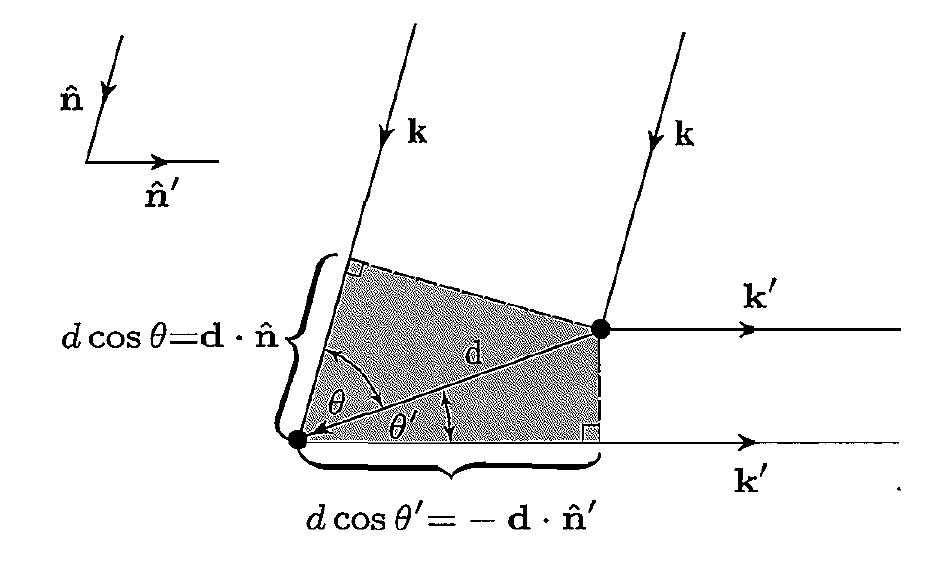
\includegraphics{../assets/theorie/lauebeugung}
    \caption{Skizze zur Erklärung der Laue-Bedingung. \imcitetwo{Ashcroft}} \label{fig:laue}
\end{figure}
Zur Herleitung der Beugungsbedingung nach Laue betrachtet man die Bestrahlung zweier Gitterpunkte mit Photonen unter
Annahme von elastischer Streuung.
Der Abstand der Gitterpunkte ist durch den Vektor $\mathbf{O}$ gegeben.
Dabei ist die einfallende Strahlung durch den Wellenzahlvektor  $\mathbf{k}$ charakterisiert.
Es gilt der Zusammenhang $\lvert \mathbf{k} \rvert = 2 \pi / \lambda$ und die Dispersionsrelation
$\omega = \c \lvert \mathbf{k} \rvert$.
Die gestreute Strahlung wird durch den Wellenzahlvektor $\mathbf{k}'$ beschrieben.
Da nur elastische Streuung betrachtet wird, gilt $\lvert \mathbf{k} \rvert=\lvert \mathbf{k}' \rvert$.
Somit sind die Frequenzen ($\omega$ und $\omega'$) beider Wellen gleich.
Für den Wegunterschied $\Delta s$ findet man anhand \cref{fig:laue} den Zusammenhang \autocite{Ashcroft}:
\begin{equation}
    \Delta s = \Delta s_{1} + \Delta s_{2} = \underbrace{ \mathbf{O} \cdot \frac{\mathbf{k}}{\lvert \mathbf{k} \rvert }
    -\mathbf{O}\cdot \frac{\mathbf{k}'}{\lvert \mathbf{k}' \rvert}  }_{\substack{\text{Projektion von } \\ \mathbf{O} \text{ auf }
    \mathbf{k} \text{ bzw. }\mathbf{k'} }} =  \frac{\lambda}{2\pi} \mathbf{O}\cdot\Delta \mathbf{k}.
    \label{eq:laue}
\end{equation}
Hierbei ist $\Delta \mathbf{k} = \mathbf{k}-\mathbf{k}'$ der Differenzvektor der Wellenzahlvektoren.
Für konstruktive Interferenz muss die Bedingung $\Delta s = n \lambda, n \in \mathbb{N}$ erfüllt sein, sodass durch
Gleichsetzen die Beziehung $\mathbf{O}\cdot\Delta \mathbf{k} =2\pi n$ folgt.
Aus der geometrischen Anordnung der Gitterpunkte ergibt sich ein Wegunterschied, der äquivalent
zu einer Phasendifferenz von $\Delta\varphi=(2\pi / \lambda) \cdot \Delta s = \Delta \mathbf{k}\cdot \mathbf{O}$ ist.

Unter der Annahme, dass beide Gitterpunkte Kugelwellen mit Amplituden $u_{0}(\mathbf{r})$ und $u_{1}(\mathbf{r})$
ausstrahlen, ergibt sich für die Überlagerung beider Wellen die folgende Form \autocite{Spiess}:
\begin{align}
    u(\mathbf{r},t)=u_{0}(\mathbf{r})\cdot \exp(\mathrm{i}\omega t+\mathrm{i}\lvert \mathbf{k}
    \rvert r) + u_{1}(\mathbf{r}) \cdot \exp(\mathrm{i}\omega t + \mathrm{i}\lvert \mathbf{k}
    \rvert r+\mathrm{i}\Delta\varphi).
\end{align}
Diese Überlagerung führt zu einer Interferenz, die durch die Phasendifferenz $\Delta\varphi$ bestimmt
wird.

\paragraph{Streuung an allen Gitterpunkten}
Will man die Streuung im gesamten Kristall betrachten, muss über alle Streuzentren, das heißt über alle Gittervektoren,
im Kristall summiert werden.
Diese sind gegeben durch $\mathbf{O}_{pqr}=p\mathbf{a}_{1}+q\mathbf{a}_{2}+r\mathbf{a}_{3}$.
Für die Superposition aller Wellen mit Amplitude $u_{pqr}(\mathbf{r})$ und Phasendifferenz $\Delta\varphi_{pqr}$
ergibt sich:
\begin{align}
    \begin{split}
        u(\mathbf{r}, t)
        &=\sum_{pqr} u_{pqr}(\mathbf{r})\cdot \exp(\mathrm{i}\omega t+\mathrm{i}
        \lvert \mathbf{k} \rvert r+\mathrm{i}\underbrace{ \Delta\varphi_{pqr} }_{ = \Delta
        \mathbf{k}\cdot \mathbf{O}_{pqr}})) \\
        &=\exp(\mathrm{i}\omega t+\mathrm{i}\lvert \mathbf{k} \rvert r)\cdot
        \underbrace{ \sum_{pqr}u_{pqr}(\mathbf{r})\cdot \exp(\mathrm{i}\Delta \mathbf{k}
        \cdot \mathbf{O}_{pqr}) }_{ \coloneqq A }.
    \end{split}
    \label{eq:amplitude}
\end{align}
Die Größe $A$ wird als Streuamplitude bezeichnet.
Die tatsächliche Streuung erfolgt an der Elektronenverteilung.
Das führt zu zusätzlichen Effekten wie dem Atomformfaktor und dem Strukturfaktor,
welche für weitere Betrachtungen jedoch vernachlässigt werden können \autocite{Spiess}:
\begin{equation}
    A \propto \int n(\mathbf{r}) \exp(\mathrm{i} \Delta \mathbf{k}\cdot
    \mathbf{r}) \, \mathrm{d}V(\mathbf{r}).
    \label{eq:atomformfaktor}
\end{equation}

\paragraph{Beugungsbedingung}
Die Bedingung für konstruktive Interferenz ist äquivalent zur Maximierung der Streuamplitude.
Damit diese maximal wird, muss die Interferenzbedingung $\mathbf{O}_{pqr}\cdot\Delta \mathbf{k} =2\pi z$
für alle $p$, $q$, $r$ gelten.
Zerlegt man $\mathbf{O}_{pqr}$ in seine Komponenten, erhält man folgende Gleichungen:
\begin{equation}
    \mathbf{a}_{1}\cdot\Delta \mathbf{k} = 2\pi h, \quad
    \mathbf{a}_{2}\cdot\Delta \mathbf{k} = 2\pi k, \quad
    \mathbf{a}_{3}\cdot\Delta \mathbf{k} = 2\pi l.
    \label{eq:lauebedingung}
\end{equation}
Dies sind die Laue-Gleichungen für Beugungsmaxima.
Sie sind erfüllt, falls $\Delta \mathbf{k}$ ein reziproker Gittervektor ist.
Es stellt die Beugungsbedingung nach Laue dar, die besagt, dass konstruktive Interferenz genau dann auftritt,
wenn $\Delta \mathbf{k}$ einem Vektor des reziproken Gitters entspricht \autocite{Ashcroft}.

Für die Strukturamplitude ergibt sich anschließend:
\begin{equation}
    A = \sum_{pqr} u_{pqr}(\mathbf{r}) \cdot\underbrace{ \exp(2\pi \mathrm{i}
    \cdot(\underbrace{ mh+nk+pl }_{ \in\mathbb{Z} })) }_{ =1 }
    = \sum_{pqr} u_{pqr}(\mathbf{r}).
    \label{eq:strukturamplitude}
\end{equation}

\paragraph{Bragg-Bedingung}
Die Bragg Bedingung kann sowohl mithilfe der Laue-Bedingung als auch geometrisch hergeleitet werden.
Um die Äquivalenz zur Laue-Bedingung zu zeigen, wird die Bragg-Bedingung im Folgenden aus der Laue-Bedingung
hergeleitet.
Betrachtet man einen Differenzvektor $\Delta \mathbf{k}=\mathbf{k}'-\mathbf{k}$, wobei $\mathbf{k}$ und
$\mathbf{k'}$ den Winkel $\alpha$ einschließen,so ist sein Betrag gegeben durch:
\begin{align}
    \begin{split}
        \lvert \Delta \mathbf{k} \rvert ^{2}&=\langle \Delta \mathbf{k} ,\Delta \mathbf{k}\rangle =\langle
        \mathbf{k}-\mathbf{k}', \mathbf{k}-\mathbf{k}' \rangle = k^{2}+k'^{2}-2kk'\cos(\alpha)  \\
        &=2{k}^{2}(1-\cos(\alpha))=4k^{2}\sin ^{2}\left( \frac{\alpha}{2} \right)
        =4k^{2}\sin ^{2}( \nu).
    \end{split}
\end{align}
Hierbei ist $\nu = \alpha / 2$ der Bragg-Winkel und $\langle \cdot , \cdot \rangle$ das Standardskalarprodukt.
Da $\Delta \mathbf{k}$ ein Vektor aus dem reziproken Raum ist und senkrecht auf der Gitterebene
steht, an welcher er gestreut wird, existiert ein kürzester Vektor $\mathbf{g}$, sodass
$n\cdot \mathbf{g} =\Delta \mathbf{k}$.
Aus \cref{subsubsec:indizierung} ist bekannt, dass $\mathbf{g}$ den Abstand der Netzebenen definiert
mit $d = 2 \pi \cdot\lvert \mathbf{g} \rvert ^{-1}$.
Daraus folgt $\lvert \Delta \mathbf{k} \rvert=n \lvert \mathbf{g} \rvert = 2\pi n/d$.
Kombiniert man beide Gleichungen miteinander, ergibt sich die Bragg-Bedingung \autocite{Ashcroft}:
\begin{align}
    \begin{split}
        2k\sin(\nu)&=\frac{2\pi n}{d}, \\
        2d\sin(\nu)&=n \lambda.
    \end{split}
\end{align}

\subsection{Entropiestabilisierte Metalloxide}\label{subsec:hochentropische-metalloxide}
\begin{figure}
    \centering
    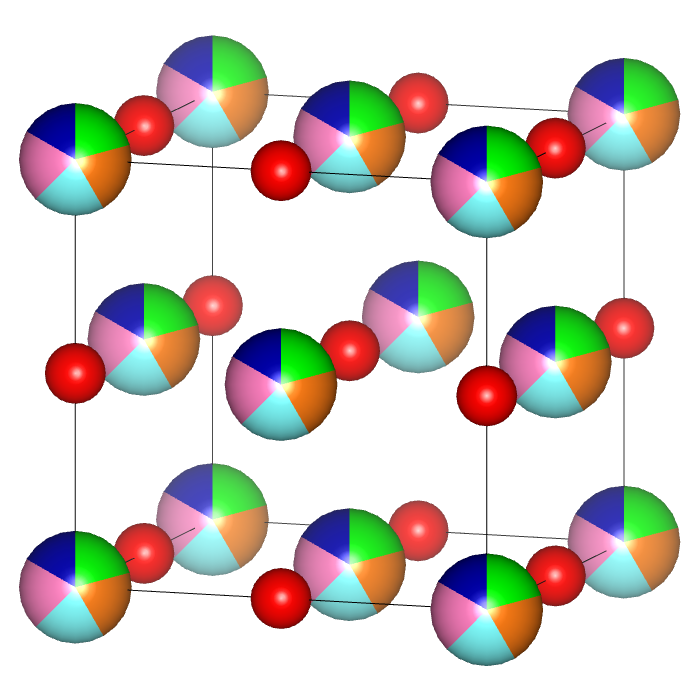
\includegraphics[width=0.3\textwidth]{../assets/theorie/heo}
    \caption{Struktur von \heo. Rot: Sauerstoff, Bunt: Metallkationen.}
    \label{fig:heo}
\end{figure}
Wie bereits in \cref{sec:einleitung} erwähnt, haben \citeauthoryear{Rost2015} eindrucksvoll eine neue Klasse von
Materialien vorgestellt, die sogenannten entropiestabilisierten Metalloxide.
Obwohl in dieser Arbeit mit Dünnfilmen gearbeitet wird, deren Eigenschaften nicht identisch mit den korrenspodierenden
Massivmaterialien sind, bietet die Forschung von \citeauthoryear{Rost2015} wertvolle Einblicke und
Vergleichsmöglichkeiten.
Im Folgenden wird aus diesem Grund die Synthese und Struktur von \heo\,-Pellets
sowie die zugrundeliegende Theorie
der Entropiestabilisierung erläutert.

\subsubsection{Synthese und Struktur von \texorpdfstring{\heo}{MgCoNiCuZnO}}\label{subsubsec:heo}
Für die Herstellung von \heo\ wurden von \citeauthoryear{Rost2015} die einzelnen binären Oxidpulver \ce{MgO}, \ce{CoO},
\ce{NiO}, \ce{CuO} und \ce{ZnO} zu äquimolaren Anteilen gemahlen, in Pellets gepresst und anschließend bei den
Temperaturen \qtylist{750;800;850;900;1000}{\celsius} für \qty{2}{\hour} gesintert.
Anschließend wurden die Proben durch direkte Extraktion aus dem Ofen auf Raumtemperatur abgekühlt.
Nach jedem Ausheizprozess wurde die Kristallinität durch Röntgendiffraktometrie untersucht.
Die Diffraktogramme sind in \cref{fig:rost1} dargestellt.
Bei den Temperaturen \qtylist{750;800;850}{\celsius} wurden mithilfe von $2\theta/\omega$-Diffraktogrammen die
Natriumchloridstruktur und die Tenoritstruktur identifiziert.
Eine vollständige Transformation in die Natriumchloridstruktur erfolgte zwischen \qty{850}{\celsius} und \qty{900}{\celsius}.

\citeauthoryear{Rost2015} stellen weitere Proben her, um die Rolle der Entropie im Bezug zur Phasenübergangstemperatur
zu charakterisieren.
Für jedes Metallkation wurde eine Serie von Proben synthetisiert, in der die Konzentration $X$ des jeweiligen
Metallkations zwischen \qty{10}{\percent} und \qty{30}{\percent} variierte und die Konzentrationen der anderen
Metallkationen äquimolar verteilt waren.
Erneut wurde die Kristallinität durch Röntgendiffraktometrie untersucht
und die Übergangstemperatur zur Einzelphase als Funktion der Konzentration $X$ bestimmt, siehe \cref{fig:rost2}.
Erkennbar ist, dass die Übergangstemperaturen zur Einzelphase steigen, sobald sich der Abstand $\lvert X-0.2 \rvert$
vergrößert.

\captionsetup{justification=justified}
\begin{figure}
    \centering
    \begin{subfigure}{0.9\textwidth}
        \centering
        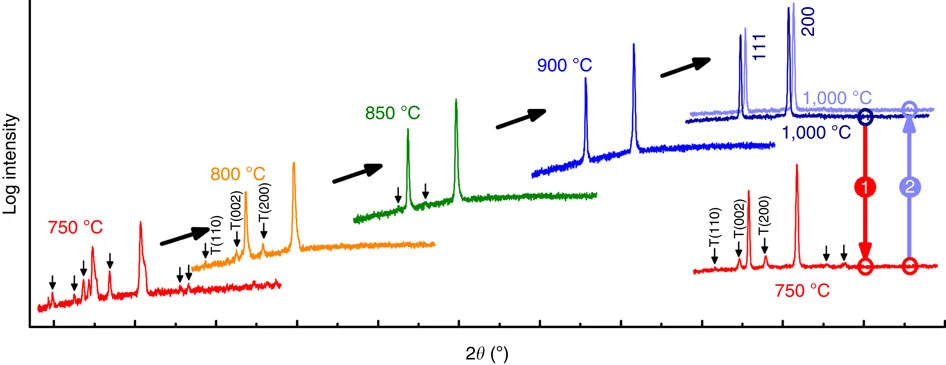
\includegraphics[width=\textwidth]{../assets/theorie/rost1}
        \caption{$2 \theta/\omega$ Diffraktogramme für \heo\ zu ausgewählten Temperaturen.
        Die Röntgenintensität ist logarithmisch aufgetragen und Pfeile zeigen auf Peaks, die mit Nicht-Natriumchloridphasen
        assoziiert sind, Peaks mit (T) und (RS) indiziert entsprechen Tenorit- bzw. Natriumchloridphasen.
        Die beiden Röntgenmuster für \qty{1000}{\degreeCelsius} geglühte Proben sind zur besseren Übersicht in
            $2\theta$ verschoben.}
        \label{fig:rost1}
        \vspace*{10mm}
    \end{subfigure}
    \begin{subfigure}{0.6\textwidth}
        \centering
        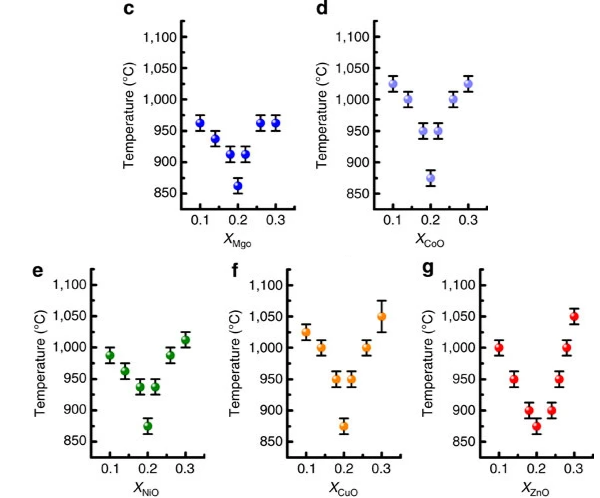
\includegraphics[width=\textwidth]{../assets/theorie/rost2}
        \caption{Partielle Phasendiagramme, welche die Übergangstemperatur zur Einzelphase als Funktion der Komposition
        in der Nähe der äquimolaren Zusammensetzung zeigen, wo maximale Konfigurationsentropie erwartet wird.
        Die Fehlerbalken berücksichtigen die Unsicherheit zwischen Temperaturintervallen. Jedes Phasendiagramm variiert
        systematisch die Konzentration eines Elements.}
        \label{fig:rost2}
        \vspace*{10mm}
    \end{subfigure}
    \caption{Auszüge aus der Arbeit von \citeauthoryear{Rost2015} \autocite{Rost2015}.}
\end{figure}
\captionsetup{justification=centering}

Diese ersten beiden Experimente weisen darauf hin, dass die Entropie eine entscheidende Rolle für die Stabilität von
\heo\ spielt.
Um dessen Struktur auf atomarer Ebene zu charakterisieren, wurden von \citeauthoryear{Rost2015} EXAFS-Messungen
und STEM-EDX Untersuchungen durchgeführt.
Die Ergebnisse legen nahe, dass \heo, in Analogie zu den HEAs, ein Mehrkomponentenoxid ist, welches in einer
Natriumchloridstruktur kristallisiert.
Dabei wird die Kationenstelle durch ein zufälliges Metallkationen \ce{Mg^{2+}}, \ce{Co^{2+}}, \ce{Ni^{2+}},
\ce{Cu^{2+}} oder \ce{Zn^{2+}} besetzt.
Im Kontrast zu den HEAs existiert ein geordnetes Anionengitter, welches durch Sauerstoffionen besetzt ist.
Die Struktur von \heo\ ist in \cref{fig:heo} dargestellt.

Es ist bemerkenswert, dass diese Phase stabil synthetisiert werden konnte, insbesondere angesichts der Änderungen in der
Kristallstruktur von \ce{ZnO} und \ce{CuO} sowie der damit verbundenen positiven Enthalpie.
Um dieses Phänomen zu verstehen, muss die Rolle der Gibbs-Energie und der darin auftretenden Entropie
erläutert werden.

\subsubsection{Gibbs-Energie und Phasenstabilität}
Aus der Thermodynamik ist bekannt, dass ein Prozess genau dann freiwillig abläuft, falls die Gesamtentropie des
Systems und seiner Umgebung zunimmt.
Beschränkt man sich auf Prozesse, die bei konstantem Druck und Temperatur ablaufen, dann ist diese Aussage äquivalent
zur Minimierung der Gibbs-Energie $G$, welche in der einfachsten Betrachtung folgendermaßen definiert ist
\autocite{Demtrder2015}:
\begin{align}
    \begin{split}
        G(T,p, \{ n_{i} \})&=H(T,p,\{ n_{i} \})-TS(T,p,\{ n_{i} \}), \\
        \Delta G(T, p, \{ n_{i} \})&=\Delta H(T,p, \{ n_{i} \})-T \Delta S(T,p, \{ n_{i} \}).
    \end{split}
    \label{eq:gibbs}
\end{align}
Hierbei ist $H$ die Enthalpie, $S$ die Entropie, $T$ die Temperatur, $p$ der Druck und $\{n_{i}\}$ die Stoffmengen jener
Komponenten, die am Prozess beteiligt sind.
Das $\Delta$ symbolisiert die Änderung der jeweiligen Größe bei Betrachtung zweier Zustände.
Die Gibbs-Energie ist eine Zustandsgröße und hängt nur von den Größen $T$, $p$ und $\{ n_{i} \}$ ab.
Die Änderung der Gibbs-Energie $\Delta G$ ist ein Maß für die Spontanität eines Prozesses.
Ist $\Delta G < 0$, so läuft der Prozess freiwillig in einen energetisch günstigeren Zustand ab \autocite{rost_phd}.
Aus dieser Forderung ist ersichtlich, dass der stabilste Zustand die Gibbs-Energie minimiert.

Die Gibbs-Energie ist maßgeblich von der Enthalpie, der Temperatur und der Entropie abhängig.
Für niedrige Temperaturen wird die Gibbs-Energie nahezu ausschließlich durch die Enthalpie bestimmt.
Nicht selten sind Enthalpie-minimierte Zustände diejenigen, die auch die Gibbs-Energie minimieren.
Für hochentropische Materialien ist das in der Regel nicht der Fall.
Diese zeichnen sich dadurch aus, dass sie eine hohe Entropie besitzen, sodass das System
bei entsprechend hohen Temperaturen in einen anderen, als den Enthalpie-minimalen Zustand übergeht \autocite{Rost2015}.
Dieser Zustand ist dann durch die Entropie stabilisiert.

In diesem Zusammenhang muss noch die Rolle des Abschreckens betrachtet werden.
Durch das schnelle Abkühlen eines Materials, beispielsweise durch das Rausnehmen einer Probe aus dem Ofen,
hat das System nicht genug Zeit, um in den Gleichgewichtszustand zu relaxieren.
Durch das Ausbilden eines lokalen Minimums in der Gibbs-Energie, welches nicht dem globalen Minimum entspricht,
kann das System in einem metastabilen Zustand verharren \autocite{rost_phd}.
Dieses Phänomen wird genutzt, um entropiestabilisierte Zustände bei hohen Temperaturen zu erzeugen
und durch Abschrecken in diesen ``einzufangen''.


\subsubsection{Mischungsentropie}
Die Entropie ist von zentraler Bedeutung in der Stabilität von hochentropischen Materialien.
Für diese Beschreibung zieht man das Modell der idealen Lösung heran.
Dies ist eine Mischung aus zwei oder mehreren Komponenten, deren Mischung nicht mit einer Änderung der
Wärme oder Volumenänderung verbunden ist \autocite{DeHoff2006}.
Dabei wird die Entropie der Mischung mithilfe der Mischungsentropie von Idealgasen beschrieben.
Für diese findet man die folgende Form \autocite{rost_phd}:
\begin{equation}
    \Delta S_{\text{Misch}} = -\mathrm{R} \sum_{i=1}^N x_{i} \ln(x_{i}).
    \label{eq:Mischungsentropie}
\end{equation}
Hierbei ist $\mathrm{R}$ die allgemeine Gaskonstante, $x_{i}$ der $i$ Stoffmengenanteil der $i$-ten Komponenten und
$N$ die Anzahl der Komponenten.
Das Maximum der Entropie wird erreicht, wenn alle Komponenten gleichmäßig verteilt sind.
Dann gilt $x_{i}=1/N$ und $\max(S_{\text{Misch}}) = \mathrm{R} \ln(N)$.

Eine weitere Möglichkeit zur Visualisierung der Mischungsentropie ergibt sich, indem man die Konzentration eines
Konstituenten variiert und alle anderen äquimolar verteilt.
Mit der Parametrisierung $x_{1} = x$ und $x_{j} = (1-x) / (N-1)$ für $j=2, \dots, N$ ergibt sich für die
Mischungsentropie \autocite{Rost2015}:
\begin{equation}
    \Delta S_{\text{Misch}} = -R \left( x \ln(x) + (1-x) \ln \left( \frac{1-x}{N-1} \right) \right).
    \label{eq:Mischungsentropie2}
\end{equation}
\begin{figure}
    \centering
    \import{../plots/theory}{mixing_entropy.pgf}
    \caption{Darstellung der Mischungsentropie in Abhängigkeit der Konzentration bei $N$ Komponenten und Variation einer
    Komponente unter äquimolarer Verteilung der übrigen Komponenten.
    Das Maxima der Mischungsentropie wird erreicht, wenn alle Komponenten gleichmäßig verteilt sind.
    \imcitetwo{Rost2015}}
    \label{fig:Mischungsentropie}
\end{figure}

Diese ist in \cref{fig:Mischungsentropie} dargestellt.
Hieraus ist erneut erkennbar, dass die Mischungsentropie maximal wird, wenn alle Komponenten äquimolar verteilt sind.

Im Bezug auf die Gibbs-Energie impliziert dies, das die für den Phasenübergang nötige Temperatur umso niedriger sein
kann, je höher die Mischungsentropie ist.
Für eine äquimolare Verteilung ist die geringste Temperatur notwendig, um den Phasenübergang zu erreichen.
Aus diesem Grund wurden die Komponenten in \heo\ äquimolar verteilt.

\subsubsection{Ideale und reale Lösungen}
Mithilfe der idealen Lösung konnte die Mischungsentropie von \heo\ beschrieben werden.
Das Problem ist, dass in diesem Modell die Enthalpie der Mischung nicht verändert wird.
Für die ideale Lösung gilt $\Delta H_\mathrm{Misch} = 0$.
In der Realität ändern sich jedoch die Bindungsenergien der Atome.
Wie in \cref{subsubsec:kristallgitter} erläutert, kristallisiert $\ce{CuO}$ in der Tenoritstruktur, $\ce{ZnO}$ in der
Wurtzitstruktur, wohingegen \heo\ in der Natriumchloridstruktur kristallisiert.
Auch die übrigen Konstituenden ändern ihre Gitterkonstanten leicht.
Die Änderungen solcher Bindungsenergien ändern die Enthalpie der Mischung und damit auch die Gibbs-Energie.
Um eine Erweiterung zu finden, die auch die Enthalpie der Mischung berücksichtigt, betrachtet man ein
Zweikomponentensystem, welches gemischt wird:
\begin{equation}
    \mathrm{A} + \mathrm{B} \longrightarrow \mathrm{AB}.
    \label{eq:reaktion}
\end{equation}
Die Mischungsentropie ist nach vorherigem Abschnitt gegeben durch:
\begin{equation}
    \Delta S_{\mathrm{mix}}=-R[x_{\mathrm{A}}\ln(x_{\mathrm{A}})+x_{\mathrm{B}}\ln(x_{\mathrm{B}})].
    \label{eq:Mischungsentropie3}
\end{equation}
Im einfachsten Modell einer realen Lösung besitzt die Mischungsenthalpie die Form \autocite{rost_phd}:
\begin{equation}
    \Delta H_{\mathrm{Misch}}= a x_{\mathrm{A}} x_{\mathrm{B}}.
    \label{eq:Mischungsenthalpie}
\end{equation}
Hierbei ist $a$ eine Konstante, die die Bindungsenergie der Mischung beschreibt.
Unter dieser Annahme wird die Enthalpie eine Kompositionsfunktion.
Je nach Vorzeichen von $a$ können entweder gleichatomige Bindungen ($a > 0$) oder ungleichatomige Bindungen
($a < 0$) enthalpisch bevorzugt sein.
In den meisten Fällen ist $a > 0$, da energetisch ungünstigere Bindungen durch die Mischung entstehen.
Der Sonderfall $a=0$ entspricht der idealen Lösung.
Somit kann eine Erweiterung der Änderung der Gibbs-Energie gefunden werden \autocite{rost_phd}:

\begin{equation}
    \Delta G_{\mathrm{Misch}}=\Delta H_{\mathrm{Misch}}-T\Delta S_{\mathrm{Misch}}=a x_{\mathrm{A}} x_{\mathrm{B}}
    +RT[x_{\mathrm{A}}\ln(x_{\mathrm{A}})+x_{\mathrm{B}}\ln(x_{\mathrm{B}})].
    \label{eq:mischgibbs}
\end{equation}

\begin{figure}
    \centering
    \import{../plots/theory}{mixing_properties.pgf}
    \caption{Darstellung von Mischungsenthalpie, Mischungsentropie und Gibbs-Energie der Mischung in Abhängigkeit der
    Konzentration.
    \imcitetwo{rost_phd}}
    \label{fig:mixing_properties}
\end{figure}

Diese Änderung, zusammen mit Enthalpie- und Entropieänderung, ist in \cref{fig:mixing_properties} dargestellt.
Es ist zu erkennen, dass für niedrige Temperaturen die Gibbs-Energie nahezu ausschließlich durch die Enthalpie bestimmt
wird.
Das Minimum bei $x=0$ beziehungsweise $x=1$ weist darauf hin, dass die Gibbs-Energie minimal ist, wenn die
Komponenten rein sind.
Erst mit steigender Temperatur beginnt die Mischungsentropie einen Einfluss auf die Gibbs-Energie zu nehmen.
Dies sorgt für eine stabile Mischphase bei hohen Temperaturen, sodass das Minimum der Gibbs-Energie bei $x=0.5$ liegt.